% =========================================================================== %
\chapter{Архитектура программной реализация}\label{chap3_soft_architecture}
% =========================================================================== %
Была проведена реорганизация исходного кода программного каркаса, в результате которой было выделено 3 модуля. Текущая структура каталогов проекта представлена на рисунке~\ref{fig:fileStructure}.
\begin{figure}[!ht]
    \centering
    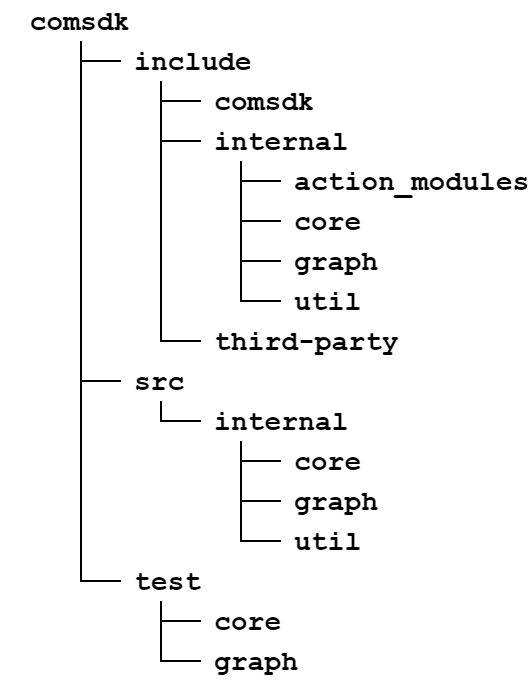
\includegraphics[height=0.35\textheight]{figures/fileStructure.png}
    \caption{Структура каталогов проекта}
    \label{fig:fileStructure}
\end{figure}
Были выделены отдельные каталоги для заголовочных файлов, где объявлены интерфейсы разработанных структур данных, и для файлов с их реализациями (\textsf{include/internal} и \textsf{src/internal} соответственно). Кроме того, создан отдельный каталог для публичных заголовочных файлов библиотеки \textsf{include/comsdk}, которые будут использоваться конечным пользователем при разработке программных реализаций различных алгоритмов.

При описании спроектированных структур данных использовался язык \glsxtrshort{UML} и были учтены возможности стандарта C++-11 языка C++.
% --------------------------------------------------------------------------- %
\section{Требования к алгоритму обхода графовых моделей}\label{sec:algorithm_task}
% --------------------------------------------------------------------------- %

Методология GBSE подразумевает параллельное независимых ветвей графа. На рисунке \ref{fig:parallelExample} после выполнения рёбер $F_{12}$~и~$F_{13}$ будет получено два независимых состояния данных $S_2$ и $S_3$ соответственно. Далее возникает задача правильным образом перевести данные из этих состояний в общее состояние $S_4$.
\begin{figure}[!ht]
    \centering
    \includegraphics[scale=0.4]{figures/example.parallel.png}
    \caption{Пример графовой модели, требующей параллельного исполнения}
    \label{fig:parallelExample}
\end{figure}

Данный подход значительно увеличивает эффективность использования ресурсов вычислительной системы и ускоряет процесс решения, однако добавляет некоторые второстепенные задачи при разработке. Так в примере на рисунке \ref{fig:parallelExample} рёбра $F_{12}$~и~$F_{13}$ выполнялись параллельно, а значит полученные в результате их выполнения данные существуют в самом общем случае в различных адресных пространствах оперативной памяти (возможно даже на двух разных вычислительных машинах). В момент разветвления графа должно происходить корректное предоставление вычислительным ресурсам (потокам, процессам, узлам кластера и т.п.) доступа к обрабатываемым данным. Помимо этого алгоритм обхода графовой модели должен корректно отрабатывать слияние ветвей графа и в частности при необходимости выполнять сбор данных.

\begin{figure}[!ht]
    \centering
    \includegraphics[scale=0.4]{figures/example.parallel_then_linear.png}
    \caption{Пример графовой модели с совмещением ветвей}
    \label{fig:parallelThenLinearExample}
\end{figure}

На рисунке \ref{fig:parallelThenLinearExample} ветви $S_1 \rightarrow S_2 \rightarrow S_4$ и $S_1 \rightarrow S_3 \rightarrow S_4$ выполняются с использованием различных вычислительных ресурсов, но ребро $F_{45}$ выполняется в пределах одной <<общей>> ветви графа $S_4 \rightarrow S_5$, и в момент его выполнения ресурсы, выделенные на выполнение двух паралельных ветвей уже не требуются. Таким образом, целесообразно разработать управляющую структуру, которая бы отвечала за выделение и освобождение вычислительных ресурсов во время работы с несколькими параллельными ветвями графа.

Кроме того, разрабатываемая архитектура должна поддерживать несколько вариантов параллельного исполнения. Среди прочих желательна поддержка:
\begin{itemize}
    \item поочерёдного выполнения (в первую очередь для отладки) в одном потоке управления;
    \item выполнения с использованием нескольких процессов операционной системы;
    \item выполнения с использованием нескольких потоков процессора;
    \item выполнения на удалённых узлах (через SSH-соединение).
\end{itemize}

Таким образом целесообразна поддержка единого интерфейса обозначенной управляющей структуры для разных режимов выполнения (последовательный, параллельный, распределённый и пр.).

В случае, когда параллельного выполнения не требуется и предусмотрено условное ветвление, оно должно быть реализовано при помощи специальных функций, привязываемых к узлам графовой модели. В контексте <<графоориентированного подхода>> такие функции называются \emph{селекторами}. Формально функция-селектор $h_i$, привязанная к узлу $v_i$, должна входному набору данных $\bar{D}$ ставить в соответствие множество рёбер $E_i$, выходящих из $v_i$, проход по которым нужно совершить. Пример работы функции-селектора демонстрирует рисунок~\ref{fig:graphSelector}.

\begin{figure}[H]
    \centering
    \includegraphics[width=\textwidth]{figures/example.selector.png}
    \caption{Пример фрагмента графовой модели с функцией-селектором}
    \label{fig:graphSelector}
\end{figure}

На рисунке~\ref{fig:graphSelector} красным обозначено ребро, переход по которому будет совершён после вызова функции-селектора.

Алгоритмы обхода графовых моделей, предусматривающие условное ветвление и параллельное выполнение ветвей представлены в разделе~\ref{sec:algorithm_task}.
% --------------------------------------------------------------------------- %
\section{Функциональные структуры данных}\label{sec:functional_classes}
% --------------------------------------------------------------------------- %
\subsection{Базовый класс}
Поскольку методология GBSE позволяет во время работы алгоритма загружать функции-предикаты, функции-обработчики и функции-селекторы из стандартных или пользовательских динамических библиотек, требовалась некоторая абстракция вида <<функция, загружаемая из динамической библиотеки>>. При анализе исходных компонентов библиотеки comsdk, было обнаружено, что такая абстракция уже реализована в классе \textsf{ActionItem}. Он представляет собой абстракцию над любой функциональной возможностью реализуемой системы. После выполнения \textsf{ActionItem} возвращется код, сообщающий об успехе или ошибке. Возможные значения кода были вынесены в отдельный перечислимый тип \textsf{ActionRetCode}. Все значения кодов приведены на рисунке~\ref{fig:UMLActionItems}. Изначально входными данными для \textsf{ActionItem} мог быть только объект класса \textsf{Anymap}, поэтому был разработан шаблон класса для поддержки различных типов входных данных. UML-диаграмма разработанных шаблонов классов предствлена на рисунке~\ref{fig:UMLActionItems}.
\begin{figure}[!ht]
    \centering
    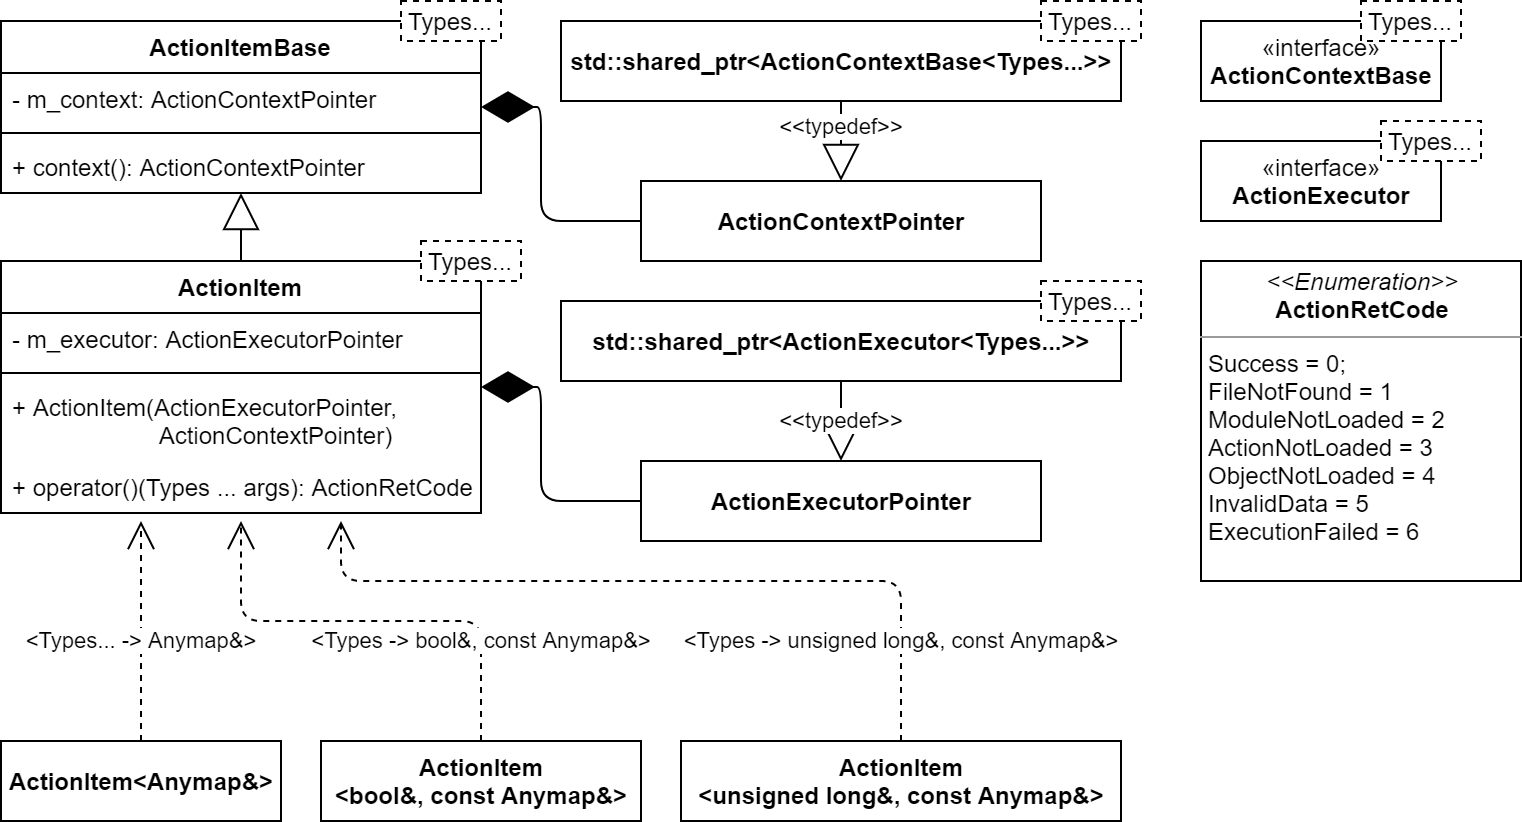
\includegraphics[width=0.95\textwidth]{figures/UML.actionItem.png}
    \caption{Структура классов, описывающих функциональные возможности системы}
    \label{fig:UMLActionItems}
\end{figure}

Запуск функциональной возможность осуществляется посредством перегруженного оператора вызова. Абстрактный класс \textsf{ActionContextBase} представляет собой интерфейс для объектов, отвечающих за запуск и хранение мета-информации о выполнении различных \textsf{ActionItem}. Базовый класс \textsf{ActionExecutor} представляет собой интерфейс для объектов, отвечающих за синхронное выполнение \textsf{ActionItem}. В исходной версии comsdk уже была реализация этого интерфейса, позволяющая выполнять загружаемые из динамических библиотек функции -- класс \textsf{SharedLibFuncExecutor}.

Для реализации обработчиков, предикатов и селекторов были созданы специализации шаблона \textsf{ActionItem}, которые были использованы в качестве базовых классов для реализуемых в дальнейшем функциональных структур данных.

\subsection{Класс предиката}
Функция-предикат должна принимать на вход данные в начальном состоянии и ставить им в соответствие логические 0 или 1. Поскольку результат выполнения \textsf{ActionItem} -- это числовой код \textsf{ActionRetCode}, то к входным данным помимо ссылки на объект класса Anymap была добавлена ссылка на переменную типа bool, куда будет сохраняться результат работы предиката. UML-диаграмма класса предиката, представлена на рисунке~\ref{fig:UMLGraphFunctions}.
\begin{figure}[!ht]
    \centering
    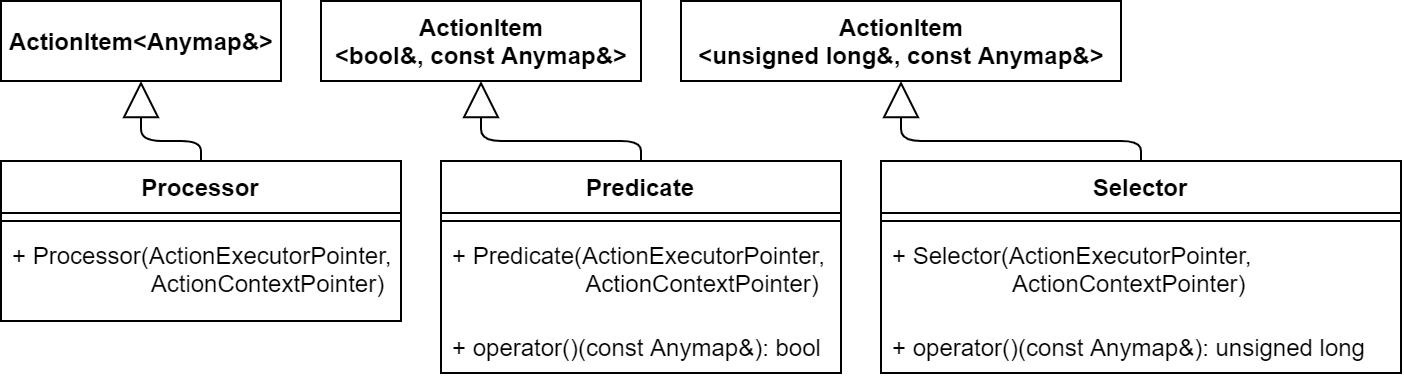
\includegraphics[width=0.95\textwidth]{figures/UML.graphFunctions.png}
    \caption{UML-диаграмма классов, описывающих функции, выполняемые при обходе графовой модели}
    \label{fig:UMLGraphFunctions}
\end{figure}

Была добавлена обёртка вокруг оператора вызова базового класса, которая возвращает переменную типа bool. Это даёт предикату интуитивно понятный интерфейс. В случае возникновения непредвиденной ошибки должно быть возвращено значение \textsf{false}.

\subsection{Класс обработчика}
Функция-обработчик отвечает за преобразование данных. Ей на вход требуется только ссылка на объект класса Anymap, содержащий обрабатываемые данные. Возвращаемым значением такой функции является код ошибки. В текущей версии класс \textsf{Processor} не расширяет базовый класс \textsf{ActionItem<Anymap\&>}, но предоставляет возможность расширения в будущем. UML-описание класса \textsf{Processor} представлено на рисунке~\ref{fig:UMLGraphFunctions}.

\subsection{Класс селектора}
Класс \textsf{Selector} должен реализовать функциональность, описанную в разделе~\ref{sec:algorithm_task}. Для описания множества рёбер, исходящих из текущей вершины, которые должны быть выполнены, были выбраны битовые маски, хранимые в одном беззнаковом целом числе (\textsf{long unsigned int}), где 1 в $i$-том справа разряде обозначает, что $i$-тое исходящее из вершины ребро должно быть выполнено. Это позволяет значительно экономить память, но ограничивает максимально возможное число исходящих рёбер разрядностью беззнаковых целых чисел. Для удобства была спроектирована обёртка над базовым оператором вызова, которая возвращает битовую маску, а не код ошибки. При возникновении исключительной ситуации должна быть возвращена битовая маска, состоящая из нулей. UML-описание класса \textsf{Selector} представлено на рисунке~\ref{fig:UMLGraphFunctions}.

\subsection{Класс функции перехода}
Задачей функции перехода является перевод данных из одного состояние в другое. Перед выполнением перехода должна выполнятся валидация данных с помощью функции-предиката. В случае успеха должна вызываться функция-обработчик. Таким образом, структура данных, описывающая функцию перехода, должна содержать в себе и функцию-предикат, и функцию-обработчик. UML-диаграмма разработанной структуры данных представлена на рисунке~\ref{fig:UMLTransfer}.
\begin{figure}[!ht]
    \centering
    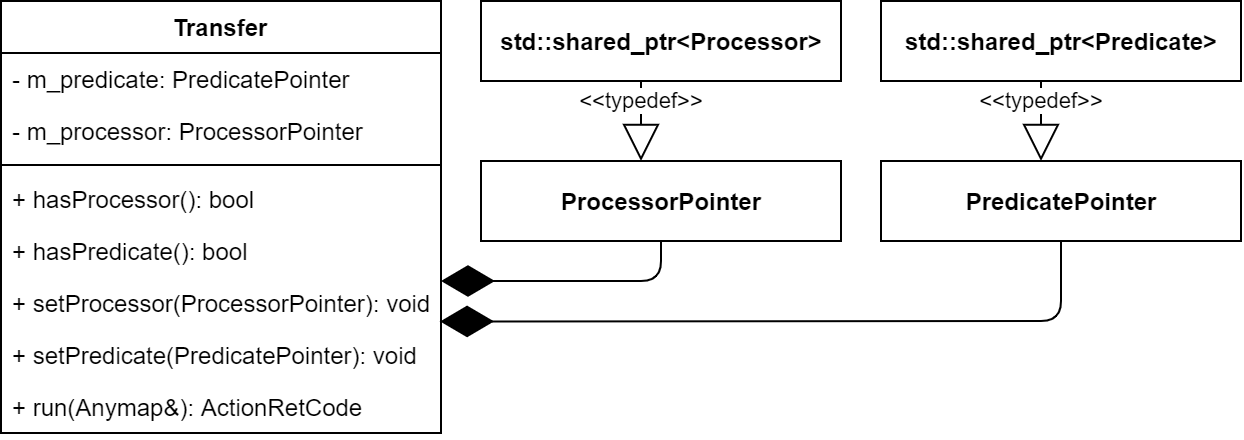
\includegraphics[width=0.90\textwidth]{figures/UML.transfer.png}
    \caption{UML-описание класса, реализующего функции перехода}
    \label{fig:UMLTransfer}
\end{figure}

Класс \textsf{Edge} хранит в себе ``умные'' указатели на объекты классов \textsf{Predicate} и \textsf{Processor}. В него встроены методы проверки наличия предиката и обработчика -- \textsf{hasPredicate()} и \textsf{hasProcessor()} соответственно -- и их задания -- \textsf{setPredicate()} и \textsf{setProcessor()}.

Таким образом, разработанные в этом разделе структуры данных необходимы для реализации логики обхода графовых моделей.

% --------------------------------------------------------------------------- %
\section{Информационные структуры данных}
% --------------------------------------------------------------------------- %
В данном разделе представлены спроектированные структуры данных, отвечающие за представление графовых моделей и их элементов.

Был разработан класс \textsf{Node} для представления узла графовой модели. Его UML-диаграмма приведена на рисунке~\ref{fig:UMLNode}.
\begin{figure}[!ht]
    \centering
    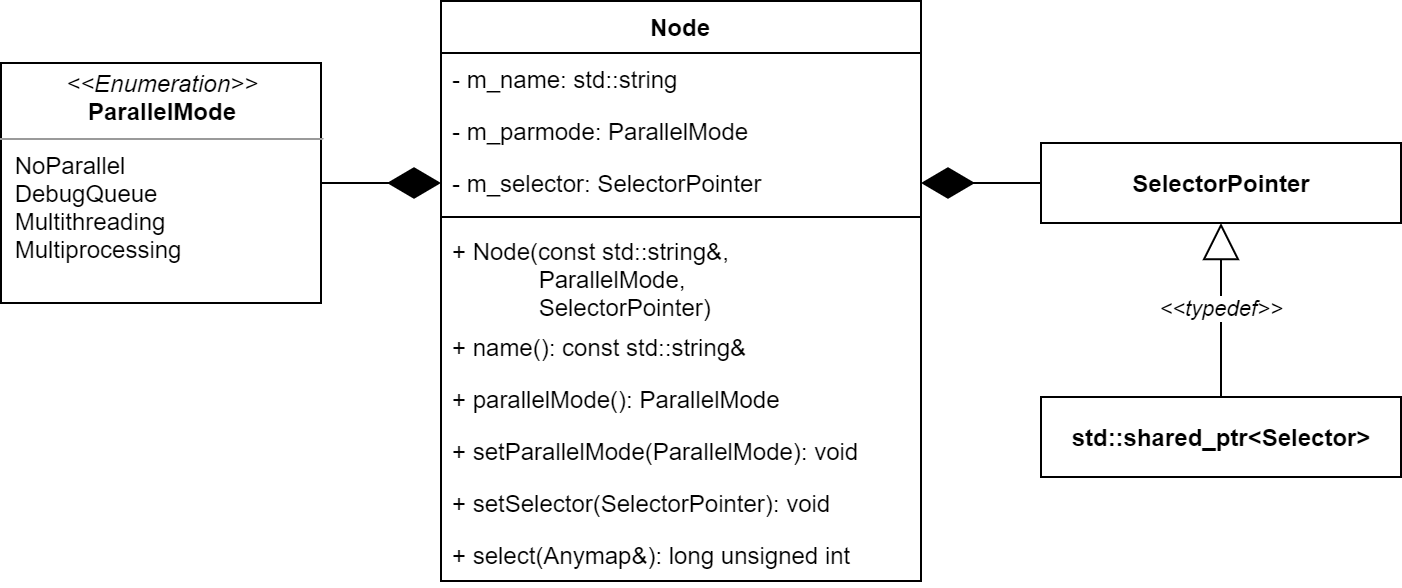
\includegraphics[height=0.25\textheight]{figures/class.node_v2.png}
    \caption{UML-описание вершины графовой модели}
    \label{fig:UMLNode}
\end{figure}

Класс \textsf{Node} хранит в себе имя вершины, режим параллельного обхода нескольких ветвей, выходящих из данной вершины и указатель на объект класса \textsf{Selector}, описанный в разделе~\ref{sec:functional_classes}. Режим параллельного обхода описан при помощи переменной перечислимого типа \textsf{ParallelMode}. В случае, когда логика алгоритма преполагает ветвление в текущей вершине, а не параллельное выполнение выходящих из неё вершин, поле \textsf{m_parmode} должно иметь значение \textsf{NoParallel}.

С рёбрами графовой модели в методологии GBSE связаны функции перехода. При этом должна быть реализована возможность в одном ребре обозначить три этапа обработки данных:
\begin{enumerate}
    \item подготовка данных;
    \item непосредственная обработка данных;
    \item пост-обработка данных.
\end{enumerate}
При проектировании структуры данных ребра графовой модели эта возможность была учтена. Описание спроектированной структуры данных приведено на рисунке~\ref{fig:UMLEdge}.
\begin{figure}[!ht]
    \centering
    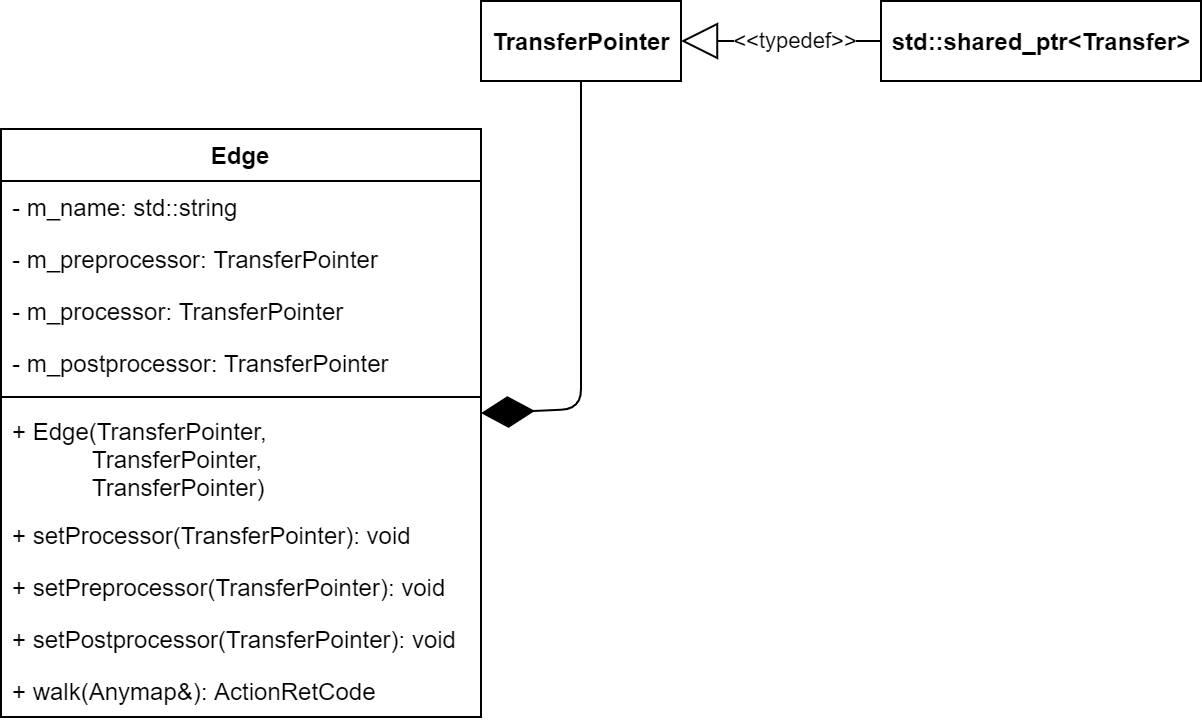
\includegraphics[height=0.27\textheight]{figures/UML.edge.png}
    \caption{UML-описание структуры данных, описывающей ребро графовой модели}
    \label{fig:UMLEdge}
\end{figure}
Конструктор класса \textsf{Edge} принимает на вход три ``умных'' указателя (\textsf{std::shared_ptr}) на объекты класса \textsf{Transfer}.
% --------------------------------------------------------------------------- %
\section{Управляющие структуры данных}
% --------------------------------------------------------------------------- %
Основной структурой данных, поддерживающей разработанный алгоритм обхода (описан в разделе~\ref{sec:algorithm_desc}) является структура данных <<контейнер выполнения>>. Задача её внутренней логики -- контролировать параллельный обход нескольких ветвей графа и отслеживать их слияние. Помимо прочего это подразумевает выделение и освобождение вычислительных ресурсов для параллельного обхода. Поскольку в общем случае могут применяться различные вычислительные ресурсы (потоки ядер процессора, процессы операционной системы, узлы вычислительного кластера и пр.), было принято решение разработать единый интерфейс структуры <<контейнер выполнения>> без привязки к конкретным ресурсам. Это позволит независимо разрабатывать различные реализации данной структуры для различных режимов параллельного обхода.

Помимо прочего при проектировании интерфейса структуры данных <<контейнер выполнения>> были задействованы разработанные информационные структуры данных <<операция с вершиной>> (\textsf{NodeOp}) и <<операция с ребром>> (\textsf{EdgeOp}).

Интерфейсы спроектированных структур данных были описаны с помощью UML-диаграмм, представленных на рисунке \ref{fig:UMLAll}.
\begin{figure}[!ht]
    \centering
    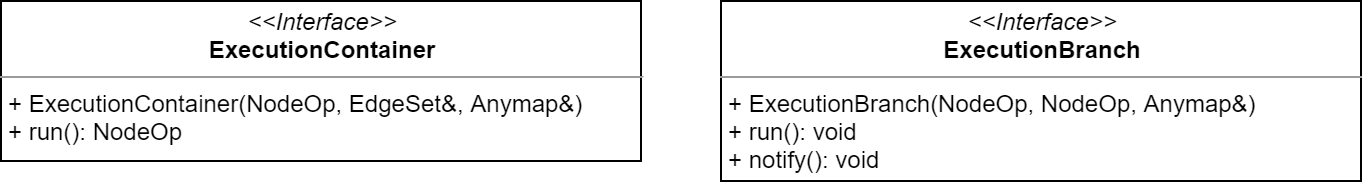
\includegraphics[width=\textwidth]{figures/UML.all.png}
    \caption{UML-диаграммы разработанных структур данных}
    \label{fig:UMLAll}
\end{figure}

Конструктор класса \textsf{ExecutionContainer} соответствует алгоритму, описанному в разделе~\ref{sec:algorithm_desc}. Метод run выполняет алгоритм, описанный блок-схемой на рисунке~\ref{fig:flowchartExecutionContainer}.

Кроме того, была спроектирован интерфейс структуры <<ветви исполнения>> (\textsf{ExecutionBranch} на рисунке~\ref{fig:UMLAll}). Её задача -- выполнение обхода одной конкретно взятой ветви (метод \textsf{run()}) графовой модели с уведомлением <<контейнера исполнения>> о завершении каждой функции перехода (метод \textsf{notify()}), как того требует алгоритм.

Таким образом, разработанные классы реализуют в себе логику параллельного обхода ветвей графовой модели и хранят данные в соответствии с разработанной процедурой обхода.

